\documentclass[%
  english,
  hyperref={pdfpagelabels=false},
  aspectratio=1610]{beamer}

\usepackage{lmodern}  % nicer fonts
\usepackage[utf8]{inputenc}
\usepackage[T1]{fontenc}

\mode<handout>{
  \usepackage{pgf}
  \usepackage{pgfpages}
  \pgfpagesuselayout{2 on 1}[a4paper,border shrink=5mm]
}
\mode<presentation>{
  \usetheme{Juelich}
}

\usepackage[english]{babel}
\usepackage[scaled]{helvet}
\usepackage{graphics}

\usepackage{listings}  % for source code display

\lstdefinelanguage{Python}{%
  morekeywords=[1]{complex,LambdaU,ForwardSendingMessaging,Sdc,QuadratureBase,GaussLobatto,Polynomial,SemiImplicitSdc},
  morekeywords=[2]{comm,prob,solver,quadr,integr,solution},
  morekeywords=[3]{communicator,nodes,weights,num_nodes,coeffs,integrator,problem,quadrature},
  sensitive=true,
  morecomment=[l]\#,
  morecomment=[l]\>,
  string=[d]\"
}
\lstset{
  language=Python,
  basicstyle=\scriptsize\ttfamily,
  commentstyle=\color{fzjgray80},
  keywordstyle=[1]\color{fzjblue50},
  keywordstyle=[2]\color{fzjgreen},
  keywordstyle=[3]\color{fzjred},
  stringstyle=\color{fzjred},
  inputencoding=utf8,
  showspaces=false,
  showstringspaces=false,
  numbers=left,
  numberstyle=\tiny\color{fzjgray80}\ttfamily,
  lineskip=0.5em
}

\usepackage{hyperref}

\title{PyPinT}
\subtitle{Towards a framework for rapid prototyping of iterative parallel-in-time algorithms}
\author{Torbjörn Klatt, Dieter Moser, Robert Speck}
\institute{3rd Workshop on Parallel-in-Time Integration}
\date{May 28, 2014}
\setbeamertemplate{slide counter}[showall]


\begin{document}
\maketitle

\begin{frame}
  \frametitle{Overview}
  \begin{enumerate}
    \item Recap of existing Parallel-in-Time Approaches\\
      {\scriptsize Parareal, (I)DC, (ML)SDC, PFASST}\\[1em]
    \item The \emph{PyPinT} Framework Explained\\
      {\scriptsize concepts, design decisions, modules}\\[1em]
    \item Goals of \emph{PyPinT}\\
      {\scriptsize creating a unicorn}\\[1em]
    \item Proof of Concept\\
      {\scriptsize coloured plots and pictures, yeah!}
  \end{enumerate}
\end{frame}


%%%%%%%%%%%%%%%%%%%%%%%%%%%%%%%%%%%%%%%%%%%%%%%%%%%%%%%%%%%%%%%%%%%%%%%%%%%%%%%%
\part{Existing Parallel-in-Time Approaches}
\makepart


\begin{frame}
  \frametitle{Parareal}
  \framesubtitle{%
    \normalfont\tiny%
    Y. Maday. 2008. \emph{The Parareal in Time Algorithm}.%
  }
  \begin{columns}[T]
    \begin{column}{4cm}
      \begin{itemize}
        \item coarse $\mathcal{\textcolor{blue}{G}}$ and fine $\mathcal{\textcolor{red}{F}}$ propagators make parareal flexible and \textcolor{fzjblue30}{modular}
        \item an initial value is improved \textcolor{fzjyellow}{iteratively}
        \item order is controllable through the fine propagator $\mathcal{\textcolor{red}{F}}$ 
      \end{itemize}
    \end{column}
    \begin{column}{8cm}
      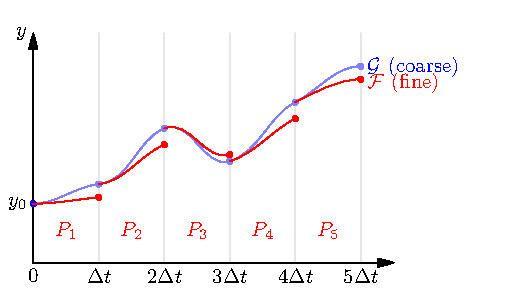
\includegraphics[width=8cm]{src/parareal_overview}
      \vspace*{-0.2cm} \hfill {\tiny [Courtesy of M.~Emmett, LBNL]}\\[0.1cm]
    \end{column}
  \end{columns}
  \begin{align*}
      \textcolor{fzjyellow}{y_{m+1}^{k+1}} = \textcolor{red}{\mathcal{F}(y_m^k)} + \textcolor{blue}{\mathcal{G}(y_m^{k+1})} - \textcolor{blue}{\mathcal{G}(y_m^k)}
  \end{align*}
  What is needed? \textcolor{fzjyellow}{Two Integrators}
\end{frame}

\begin{frame}
  \frametitle{Deferred Corrections \hspace{2em} \onslide<2>{ {\normalfont and} \hspace{2em}  Integral Deferred Corrections}}
  \framesubtitle{
    \normalfont\tiny
    \alt<1>{V. Pereyra. 1966. \emph{On Improving an Approximate Solution of a Functional Equation by Deferred Corrections}. Numerische Mathematik. 8(4) 376–391.}
           {A. Dutt, L. Greengard, V. Rokhlin. 2000. \emph{Spectral Deferred Correction Methods for Ordinary Differential Equations}. BIT Numerical Mathematics 40(2) 241–266.}%
  }
  \begin{columns}[T]
    \begin{column}{7cm}
      $ y'(t) = f\left( t, y\left( t \right) \right),\quad y\left( 0 \right)= y_{0} $\\[1.5em]
      Using the residual\\[1em]
      $r(t) = f\left( t, \tilde y\left( t \right) \right) - \tilde y'\left( t \right)$\\[1em]
      to compute the error
      \begin{align*}
        e'(t) &= f(t,\tilde y + e) - f\left( t, \tilde y \right) + r'\left( t \right)\\
        e(0)  &= 0
      \end{align*}
      for the next update
      \begin{align*}
        \tilde y_{j+1} = \tilde y_{j} + e_{j}
      \end{align*}
    \end{column}
    \begin{column}{7cm}

      \onslide<2>{
        $   y(t) = y_0 + \int_{0}^{t}  f\left( \tau, y\left( \tau \right) \right) \mathrm{d}\tau, \quad y\left( 0 \right)= y_{0} $ \\[1.5em]
        Using the residual\\[1em]
        $r(t) = y_{0} - \tilde y\left( t \right) + \int_{0}^{t} f\left(\tau, y\left( \tau \right) \right)  \mathrm{d}\tau $\\[1em]
        to compute the error
        \begin{align*}
          e(t) = \int_{0}^{t}f(\tau,\tilde y + e) - f\left( \tau, \tilde y \right) \mathrm{d}\tau + r\left( t \right)
        \end{align*}\\[0.5em]
        for the next update
        \begin{align*}
          \tilde y_{j+1} = \tilde y_{j} + e_{j}
        \end{align*}
      }
    \end{column}
  \end{columns}
\end{frame}

\begin{frame}
  \frametitle{ Spectral Deferred Corrections }
  \framesubtitle{
    \normalfont\tiny%
    A. Dutt, L. Greengard, V. Rokhlin. 2000. \emph{Spectral Deferred Correction Methods for Ordinary Differential Equations}. BIT Numerical Mathematics 40(2) 241–266.%
  }
  \begin{center}
    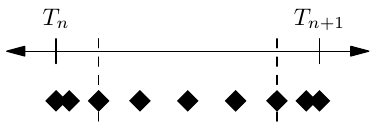
\includegraphics[width=6cm]{src/sdc_time_domain} 
  \end{center}

  One sweep is performed by
  \begin{align*}
    u_{n+1}^{k+1} = u_{n}^{k+1} + \Delta t \left[ F\left( u_{n+1}^{k+1} \right) - F\left(u_{n+1}^{k}  \right)) \right] +\mathcal{I}_{n}^{n+1}\left( F\left( \mathbf{u}^{k} \right) \right) 
  \end{align*}
  new main constituent is the quadrature operator
  \begin{align*}
    \mathcal{I}_{n}^{n+1} \mathbf{y} = \sum_{i=1}^{m} \omega_{i} \tilde y_i \approx \int_{t_n}^{t_{n+1}} y\left( \tau \right) \mathrm{d} \tau
  \end{align*}

  What is needed? \textcolor{fzjyellow}{Quadrature},  \textcolor{fzjyellow}{Evaluation of $F$} (, \textcolor{fzjyellow}{Space Solver}) $\longrightarrow$ \textcolor{fzjyellow}{new Integrator}
\end{frame}

\begin{frame}
  \frametitle{Multilevel SDC}
  \framesubtitle{%
    \normalfont\tiny%
    R. Speck, D. Ruprecht, M. Emmett, M. L. Minion, M. Bolten, R. Krause. 2013. \emph{A Multi-Level Spectral Deferred Correction Method}. arXiv Math Numerical Analysis.%
  }
  \center Slightly different sweep
  \begin{align*}
    u_{n+1}^{k+1} = u_{n}^{k+1} + \Delta t \left[ F\left( u_{n+1}^{k+1} \right) - F\left(u_{n+1}^{k}  \right)) \right] +\mathcal{I}_{n}^{n+1}\left( F\left( \mathbf{u}^{k} \right) \right) + \textcolor{fzjblue30}{\tau_{n}^{k}}
  \end{align*}
  \center and multiple level, correction $\textcolor{fzjblue30}{\tau_{n}^{k}}$ based on information from different levels\\[1.5em]
  \begin{columns}[T]
    \begin{column}{5cm}
      What is needed? 
      \begin{itemize}
        \item same as SDC
        \item \textcolor{fzjyellow}{Interpolation} {\scriptsize (space and time)}
        \item \textcolor{fzjyellow}{Restriction} {\scriptsize (space and time)}
      \end{itemize}
    \end{column}
    \begin{column}{7cm}
      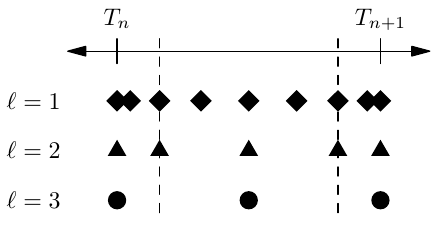
\includegraphics[width=6cm]{src/mlsdc_time_domain}
    \end{column}
  \end{columns}
\end{frame}


\begin{frame}
  \frametitle{PFASST}
  \framesubtitle{Building Blocks}
  
  \begin{picture}(1,1)
    \put(50,-125){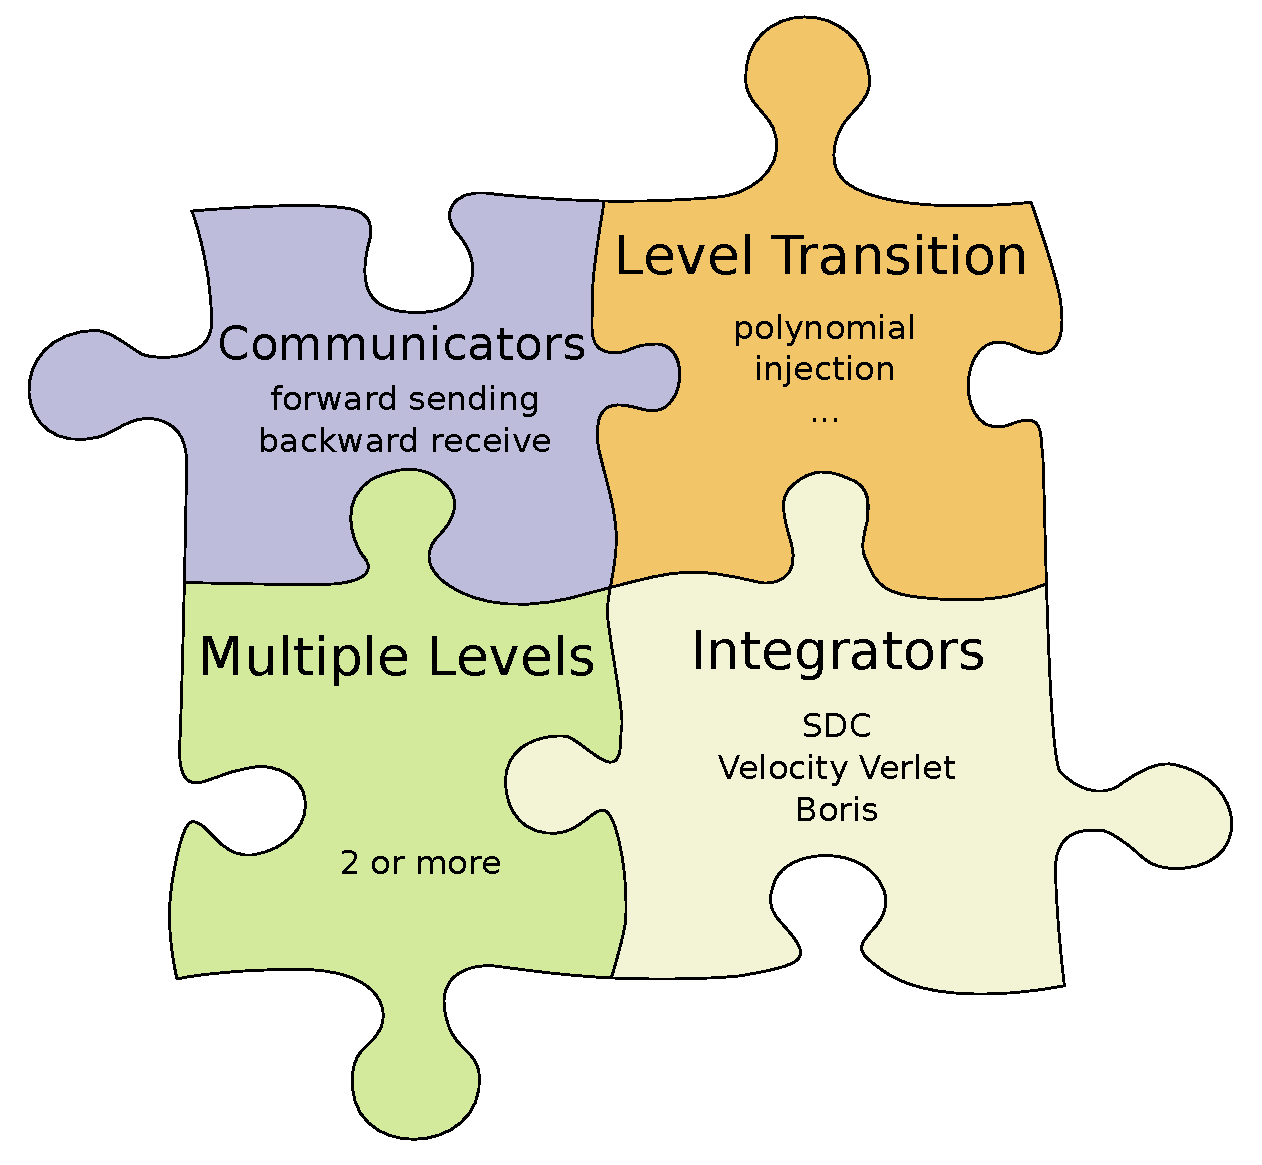
\includegraphics[height=9.5cm]{src/pfasst_blocks.pdf}}
  \end{picture}
\end{frame}


%%%%%%%%%%%%%%%%%%%%%%%%%%%%%%%%%%%%%%%%%%%%%%%%%%%%%%%%%%%%%%%%%%%%%%%%%%%%%%%%
\part{The PyPinT Framework Explained}
\makepart

\begin{frame}
  \frametitle{Basic Concept}
  \begin{itemize}
    \item \emph{Python} {\color{fzjgray80}\scriptsize $\geq$3.2} as language of choice\\
      {\scriptsize for ease of use and extensibility (cf. \emph{NumPy}, \emph{SciPy})}
    \item modular building blocks\\
      {\scriptsize for fast exchange of algorithms' building blocks}
    \item well-conceived and intuitive abstract interfaces\\
      {\scriptsize for reusable code ensuring DRY principle}
    \item integrated analyzation tools\\
      {\scriptsize for introspection and plotting (cf. \emph{matplotlib})}
    \item usage of a sophisticated unit-testing framework\\
      {\scriptsize nobody writes bug-free code}
  \end{itemize}
  
  \begin{picture}(1,1)
    \put(260,150){
\includegraphics[height=1.25cm]{src/python_logo.png}}
    \put(290,135){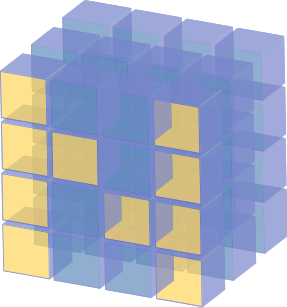
\includegraphics[height=0.75cm]{src/numpy_logo.png}}
    \put(325,135){
\includegraphics[height=0.75cm]{src/scipy_logo.png}}
    \put(290,70){
\includegraphics[height=1.1cm,angle=50]{src/puzzle_no_text.pdf}}
    \put(255,50){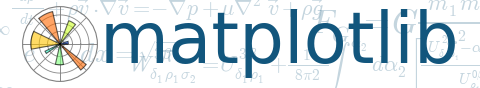
\includegraphics[height=0.75cm]{src/matplotlib_logo.png}}
  \end{picture}
\end{frame}

\begin{frame}
  \frametitle{Modules}
  \framesubtitle{Abstract Modelling of PinT Algorithms}
  \vspace{-5em}
  \begin{columns}[T]
    \begin{column}{5cm}
      \color{fzjblue50}%
      \texttt{pypint}\\
      \color{fzjgray30}%
      \hspace{0.75em}\texttt{\textasciitilde.problems}\\
      \hspace{0.75em}\texttt{\textasciitilde.solvers}\\
      \hspace{0.75em}\texttt{\textasciitilde.integrators}\\
      \hspace{0.75em}\texttt{\textasciitilde.communicators}\\
      \hspace{0.75em}\texttt{\textasciitilde.multi\_level\_providers}\\
      \hspace{0.75em}\texttt{\textasciitilde.solutions}\\
      \hspace{0.75em}\texttt{\textasciitilde.plugins}
    \end{column}
    \begin{column}{10cm}      
      \begin{picture}(1,1)
        \put(15,-175){
\includegraphics[width=6cm,angle=50]{src/puzzle_no_text.pdf}}
      \end{picture}
    \end{column}
  \end{columns}
\end{frame}

\begin{frame}
  \frametitle{Modules}
  \framesubtitle{Abstract Modelling of PinT Algorithms}
  \vspace{-5em}
  \begin{columns}[T]
    \begin{column}{5cm}
      \color{fzjblue50}%
      \texttt{pypint}\\
      \color{fzjblue50}%
      \hspace{0.75em}\texttt{\textasciitilde.problems}\\
      \color{fzjgray30}%
      \hspace{0.75em}\texttt{\textasciitilde.solvers}\\
      \hspace{0.75em}\texttt{\textasciitilde.integrators}\\
      \hspace{0.75em}\texttt{\textasciitilde.communicators}\\
      \hspace{0.75em}\texttt{\textasciitilde.multi\_level\_providers}\\
      \hspace{0.75em}\texttt{\textasciitilde.solutions}\\
      \hspace{0.75em}\texttt{\textasciitilde.plugins}
    \end{column}
    \begin{column}{10cm}
      \begin{itemize}
        \item interfaces for problem setups
        \item generic problem with specializations via mixins
      \end{itemize}
      
      \begin{picture}(1,1)
        \put(25,-120){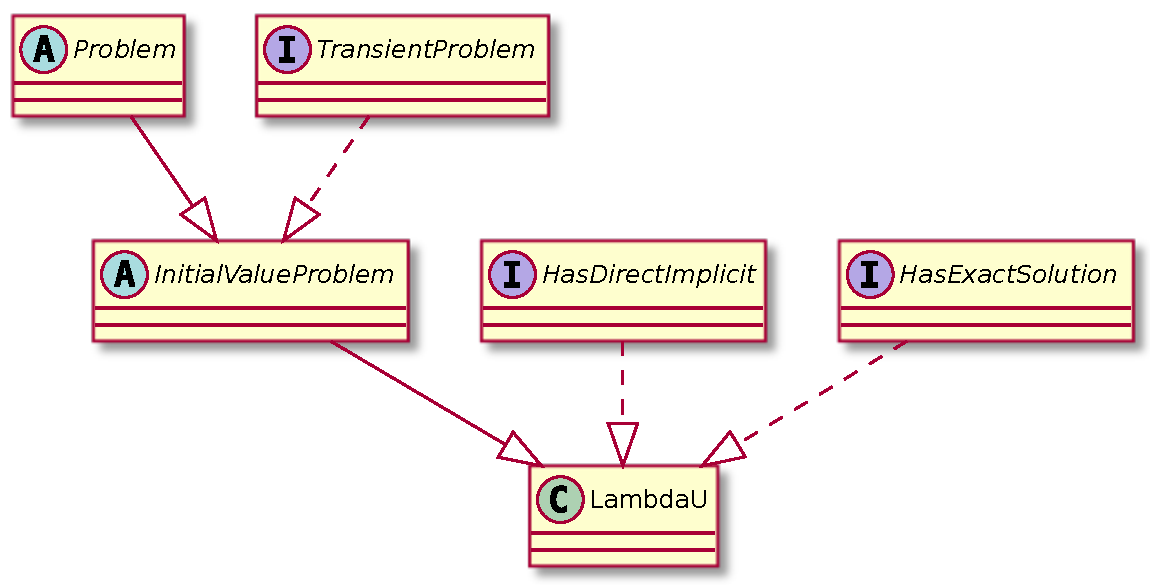
\includegraphics[width=8.5cm]{src/problem_interfaces.pdf}}
      \end{picture}
    \end{column}
  \end{columns}
\end{frame}

\begin{frame}
  \frametitle{Modules}
  \framesubtitle{Abstract Modelling of PinT Algorithms}
  \vspace{-5em}
  \begin{columns}[T]
    \begin{column}{5cm}
      \color{fzjblue50}%
      \texttt{pypint}\\
      \color{fzjgray30}%
      \hspace{0.75em}\texttt{\textasciitilde.problems}\\
      \color{fzjblue50}%
      \hspace{0.75em}\texttt{\textasciitilde.solvers}\\
      \color{fzjgray30}%
      \hspace{0.75em}\texttt{\textasciitilde.integrators}\\
      \hspace{0.75em}\texttt{\textasciitilde.communicators}\\
      \hspace{0.75em}\texttt{\textasciitilde.multi\_level\_providers}\\
      \hspace{0.75em}\texttt{\textasciitilde.solutions}\\
      \hspace{0.75em}\texttt{\textasciitilde.plugins}
    \end{column}
    \begin{column}{10cm}
      \begin{itemize}
        \item interfaces for iterative time solvers
        \item providing generic building blocks of solvers
      \end{itemize}
      
      \begin{picture}(1,1)
        \put(50,-125){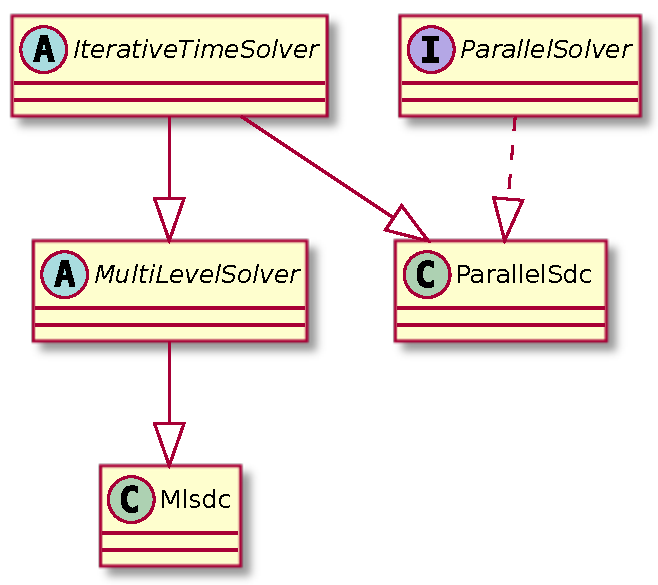
\includegraphics[height=4.5cm]{src/solvers_interfaces.pdf}}
      \end{picture}
    \end{column}
  \end{columns}
\end{frame}

\begin{frame}
  \frametitle{Modules}
  \framesubtitle{Abstract Modelling of PinT Algorithms}
  \vspace{-5em}
  \begin{columns}[T]
    \begin{column}{5cm}
      \color{fzjblue50}%
      \texttt{pypint}\\
      \color{fzjgray30}%
      \hspace{0.75em}\texttt{\textasciitilde.problems}\\
      \hspace{0.75em}\texttt{\textasciitilde.solvers}\\
      \color{fzjblue50}%
      \hspace{0.75em}\texttt{\textasciitilde.integrators}\\
      \color{fzjgray30}%
      \hspace{0.75em}\texttt{\textasciitilde.communicators}\\
      \hspace{0.75em}\texttt{\textasciitilde.multi\_level\_providers}\\
      \hspace{0.75em}\texttt{\textasciitilde.solutions}\\
      \hspace{0.75em}\texttt{\textasciitilde.plugins}
    \end{column}
    \begin{column}{10cm}
      \begin{itemize}
        \item abstract interface for integrators of ODEs\\
          {\scriptsize e.g. \emph{Runge-Kutta}, \emph{Expl./Impl. Euler}, \emph{SDC} etc.\\}
        \item unified generic interface for executing integrator\\
          {\scriptsize via method \texttt{.apply(*args, **kwargs)}}
      \end{itemize}
      
      \begin{picture}(1,1)
        \put(25,-90){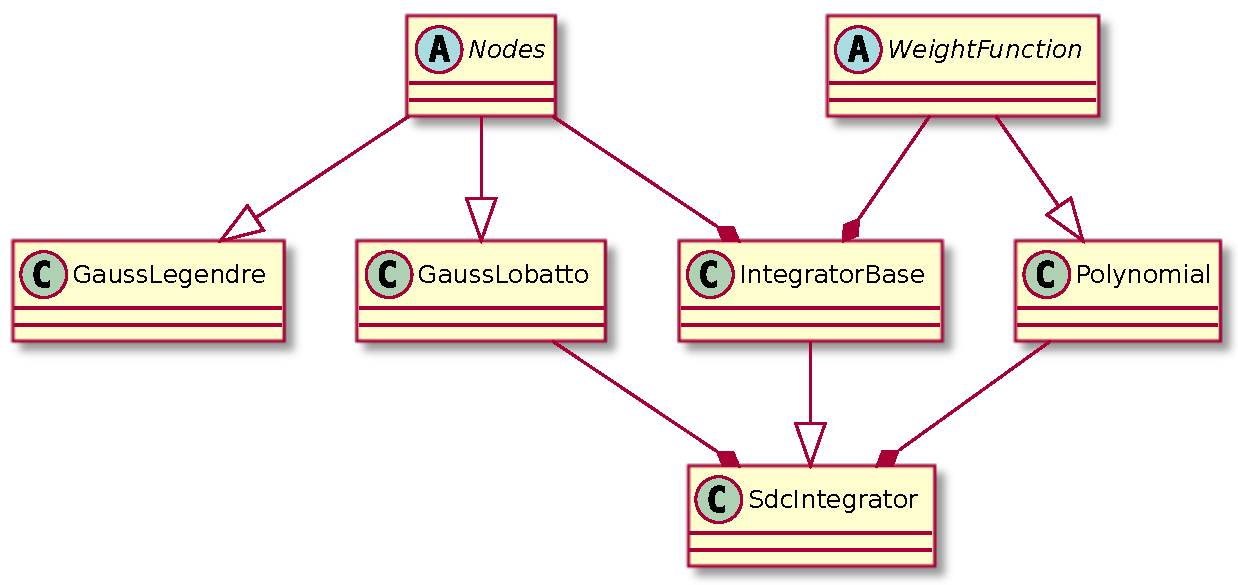
\includegraphics[height=3.5cm]{src/integrators_interfaces.pdf}}
      \end{picture}
    \end{column}
  \end{columns}
\end{frame}

\begin{frame}
  \frametitle{Modules}
  \framesubtitle{Abstract Modelling of PinT Algorithms}
  \vspace{-5em}
  \begin{columns}[T]
    \begin{column}{5cm}
      \color{fzjblue50}%
      \texttt{pypint}\\
      \color{fzjgray30}%
      \hspace{0.75em}\texttt{\textasciitilde.problems}\\
      \hspace{0.75em}\texttt{\textasciitilde.solvers}\\
      \hspace{0.75em}\texttt{\textasciitilde.integrators}\\
      \color{fzjblue50}%
      \hspace{0.75em}\texttt{\textasciitilde.communicators}\\
      \color{fzjgray30}%
      \hspace{0.75em}\texttt{\textasciitilde.multi\_level\_providers}\\
      \hspace{0.75em}\texttt{\textasciitilde.solutions}\\
      \hspace{0.75em}\texttt{\textasciitilde.plugins}
    \end{column}
    \begin{column}{10cm}
      \begin{itemize}
        \item generic abstract interfaces for communication patterns\\
          {\scriptsize e.g. implemented as \emph{forward sending}, etc.\\}
        \item extendable basic message buffer\\
          {\scriptsize holding data, solver flags and other meta information\\}
      \end{itemize}
      
      \begin{picture}(1,1)
        \put(50,-75){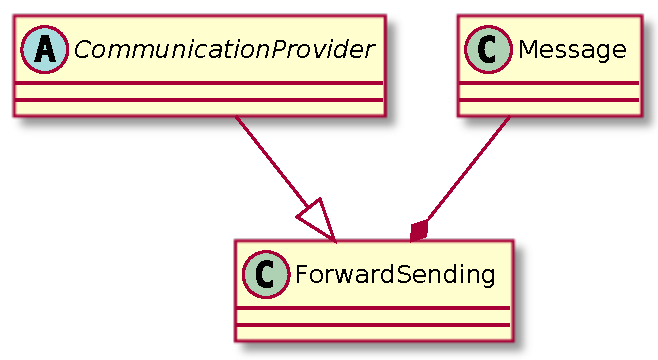
\includegraphics[height=2.5cm]{src/communicators_interfaces.pdf}}
      \end{picture}
    \end{column}
  \end{columns}
\end{frame}

\begin{frame}
  \frametitle{Modules}
  \framesubtitle{Abstract Modelling of PinT Algorithms}
  \vspace{-5em}
  \begin{columns}[T]
    \begin{column}{5cm}
      \color{fzjblue50}%
      \texttt{pypint}\\
      \color{fzjgray30}%
      \hspace{0.75em}\texttt{\textasciitilde.problems}\\
      \hspace{0.75em}\texttt{\textasciitilde.solvers}\\
      \hspace{0.75em}\texttt{\textasciitilde.integrators}\\
      \hspace{0.75em}\texttt{\textasciitilde.communicators}\\
      \color{fzjblue50}%
      \hspace{0.75em}\texttt{\textasciitilde.multi\_level\_providers}\\
      \color{fzjgray30}%
      \hspace{0.75em}\texttt{\textasciitilde.solutions}\\
      \hspace{0.75em}\texttt{\textasciitilde.plugins}
    \end{column}
    \begin{column}{10cm}
      \begin{itemize}
        \item abstract interface for generic level transitions\\
          {\scriptsize e.g. \emph{full weighting}, \emph{injection}, \emph{Lagrange-polynomial integration} etc.\\}
        \item containers for multiple levels\\
          {\scriptsize providing access to integrators of each level\\}
        \item unified generic interface for transitions between levels\\
          {\scriptsize via methods \texttt{.restrict(data, fine\_id, coarse\_id)} and\\[-0.5em]
           \texttt{.prolongate(data, coarse\_id, fine\_id)}}
      \end{itemize}
      
      \begin{picture}(1,1)
        \put(25,-85){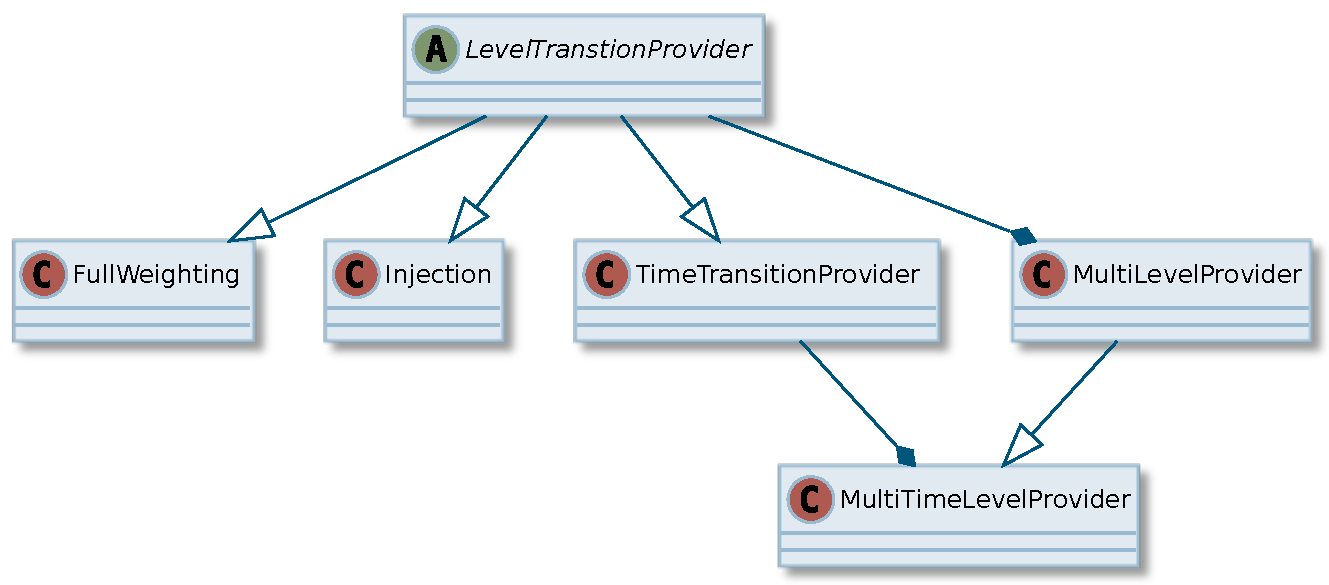
\includegraphics[height=3.5cm]{src/multi_level_providers_interfaces.pdf}}
      \end{picture}
    \end{column}
  \end{columns}
\end{frame}

\begin{frame}
  \frametitle{Modules}
  \framesubtitle{Abstract Modelling of PinT Algorithms}
  \vspace{-5em}
  \begin{columns}[T]
    \begin{column}{5cm}
      \color{fzjblue50}%
      \texttt{pypint}\\
      \color{fzjgray30}%
      \hspace{0.75em}\texttt{\textasciitilde.problems}\\
      \hspace{0.75em}\texttt{\textasciitilde.solvers}\\
      \hspace{0.75em}\texttt{\textasciitilde.integrators}\\
      \hspace{0.75em}\texttt{\textasciitilde.communicators}\\
      \hspace{0.75em}\texttt{\textasciitilde.multi\_level\_providers}\\
      \color{fzjblue50}%
      \hspace{0.75em}\texttt{\textasciitilde.solutions}\\
      \color{fzjgray30}%
      \hspace{0.75em}\texttt{\textasciitilde.plugins}
    \end{column}
    \begin{column}{10cm}
      \begin{itemize}
        \item containers for solution data + meta information\\
          {\scriptsize e.g. time-node/step-wise, trajectory (consecutive time nodes)\\}
        \item container interface for complete solutions\\
          {\scriptsize e.g. only last time node of last iteration or all nodes of all iterations\\}
      \end{itemize}
      
      \begin{picture}(1,1)
        \put(60,-115){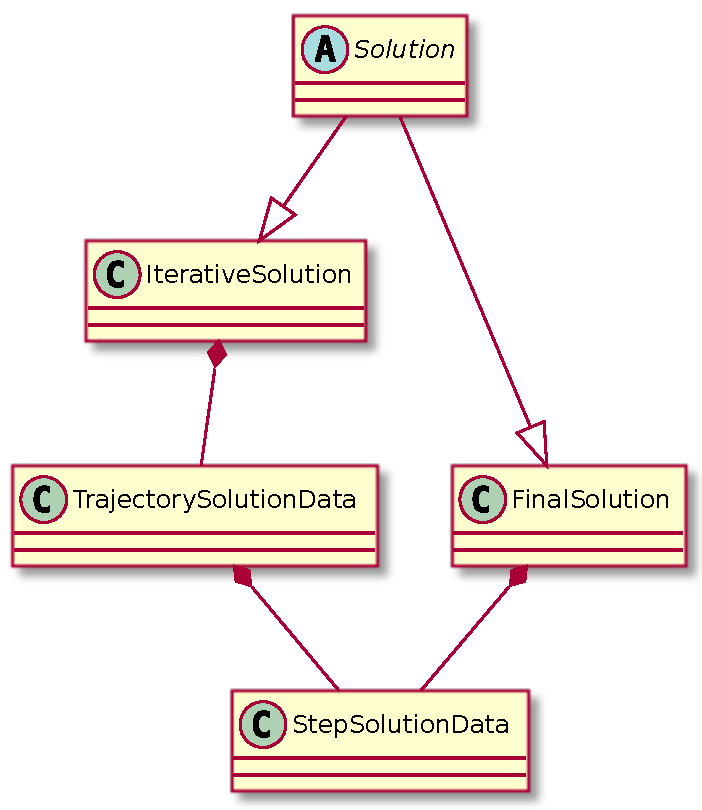
\includegraphics[height=4.5cm]{src/solutions_interfaces.pdf}}
      \end{picture}
    \end{column}
  \end{columns}
\end{frame}

\begin{frame}
  \frametitle{Modules}
  \framesubtitle{Abstract Modelling of PinT Algorithms}
  \vspace{-5em}
  \begin{columns}[T]
    \begin{column}{5cm}
      \color{fzjblue50}%
      \texttt{pypint}\\
      \color{fzjgray30}%
      \hspace{0.75em}\texttt{\textasciitilde.problems}\\
      \hspace{0.75em}\texttt{\textasciitilde.solvers}\\
      \hspace{0.75em}\texttt{\textasciitilde.integrators}\\
      \hspace{0.75em}\texttt{\textasciitilde.communicators}\\
      \hspace{0.75em}\texttt{\textasciitilde.multi\_level\_providers}\\
      \hspace{0.75em}\texttt{\textasciitilde.solutions}\\
      \color{fzjblue50}%
      \hspace{0.75em}\texttt{\textasciitilde.plugins}
    \end{column}
    \begin{column}{10cm}
      \begin{itemize}
        \item containers for solution data + meta information\\
          {\scriptsize e.g. time-node/step-wise, trajectory (consecutive time nodes)\\}
        \item container interface for complete solutions\\
          {\scriptsize e.g. only last time node of last iteration or all nodes of all iterations\\}
      \end{itemize}
      
      \begin{picture}(1,1)
        \put(10,-100){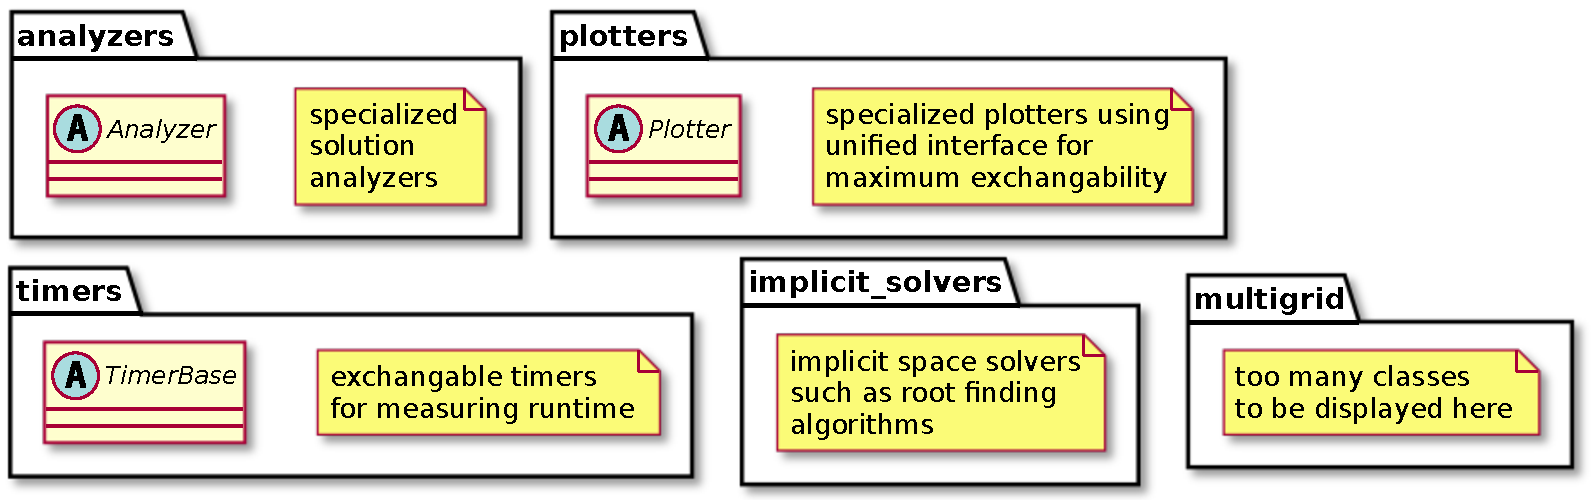
\includegraphics[width=9cm]{src/plugins_tree.pdf}}
      \end{picture}
    \end{column}
  \end{columns}
\end{frame}


%%%%%%%%%%%%%%%%%%%%%%%%%%%%%%%%%%%%%%%%%%%%%%%%%%%%%%%%%%%%%%%%%%%%%%%%%%%%%%%%
\part{Goals for PyPinT}
\makepart

\begin{frame}
  \frametitle{Goals for PyPinT}
  
  \begin{itemize}
    \item<1-> providing generic framework for many PinT algorithms\\
      {\onslide<2->\color{fzjblue50}$\Rightarrow$ easy comparability of different algorithms' building blocks\\[1.5em]}
    \item<3-> intuitive user-expandability through well-defined interfaces\\
      {\onslide<4->\color{fzjblue50}$\Rightarrow$ fast exchangability and prototyping of different building blocks\\[1.5em]}
    \item<5-> well-tested and well-documented implementations of PinT algorithms\\
      {\onslide<6->\color{fzjblue50}$\Rightarrow$ suited for educational use\\[1.5em]}
    \item<7-> open-source hosted on 
\includegraphics[height=1em]{src/GitHub-Mark-32px.png}~GitHub\\
      {\onslide<8->\color{fzjblue50}$\Rightarrow$ reaching young \& rising developers and scientists promoting PinT algorithms\\[1.5em]}
  \end{itemize}
\end{frame}


%%%%%%%%%%%%%%%%%%%%%%%%%%%%%%%%%%%%%%%%%%%%%%%%%%%%%%%%%%%%%%%%%%%%%%%%%%%%%%%%
\part{Proof of Concept}
\makepart

\begin{frame}
  \frametitle{Implementation of SDC and MLSDC}
  \framesubtitle{\normalfont Convergence Regions {\tiny\color{fzjgray50}(number iterations for residual $\leq10^{-14}$)} of $u'(x,t)=\lambda u(x,t)$, $t\in[0,1], \lambda\in\mathbb{C}$}
  \begin{center}
    \vspace{-1em}
    {\color{fzjblue50}SDC}
  \end{center}
  \begin{columns}[T]
    \begin{column}{4cm}
      \begin{picture}(1,1)
        \put(28,10){\tiny $3$ Gauss-Lobatto nodes}
        \put(-13,-95){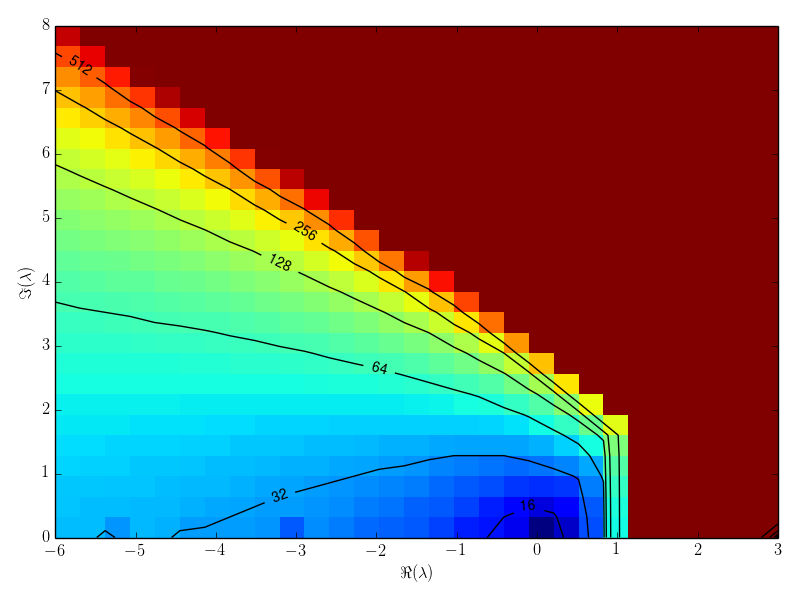
\includegraphics[height=3.5cm]{src/sdc_n3.png}}
      \end{picture}
    \end{column}
    \begin{column}{4cm}
      \begin{picture}(1,1)
        \put(28,10){\tiny $5$ Gauss-Lobatto nodes}
        \put(-13,-95){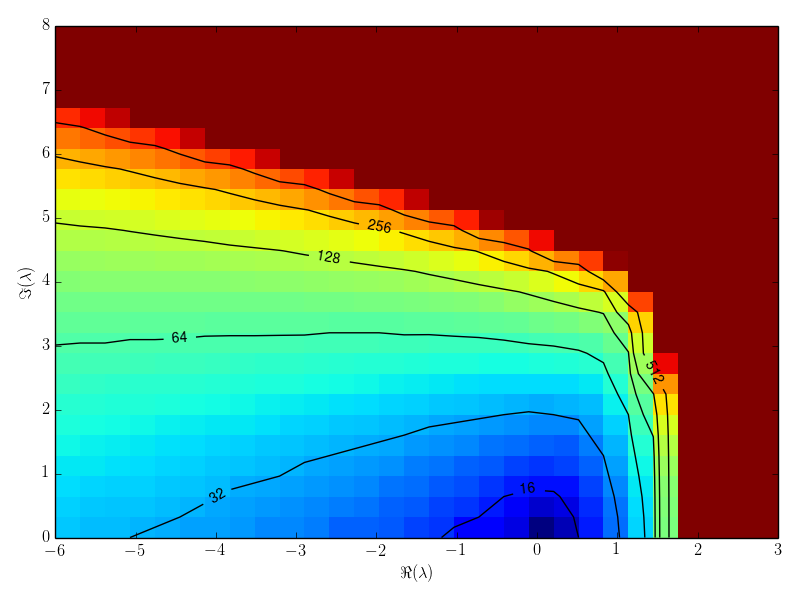
\includegraphics[height=3.5cm]{src/sdc_n5.png}}
      \end{picture}
    \end{column}
    \begin{column}{4cm}
      \begin{picture}(1,1)
        \put(28,10){\tiny $7$ Gauss-Lobatto nodes}
        \put(-13,-95){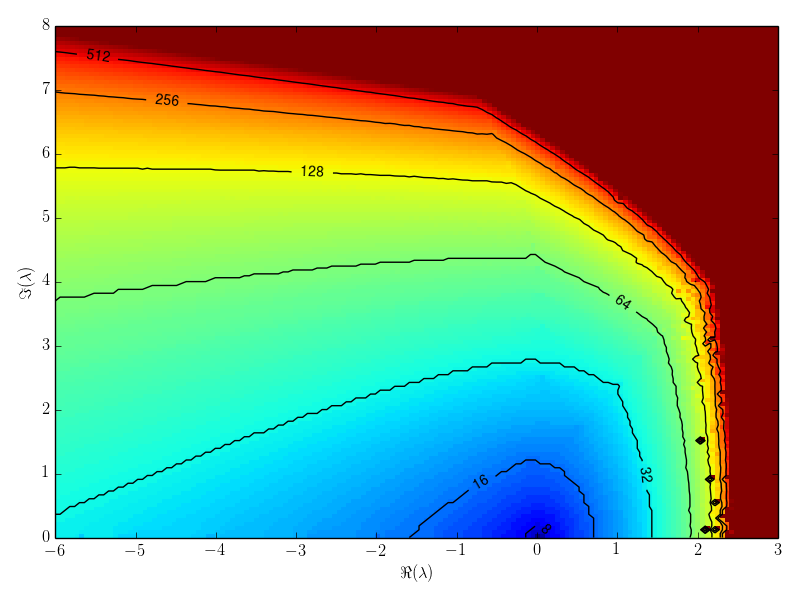
\includegraphics[height=3.5cm]{src/sdc_n7.png}}
      \end{picture}
    \end{column}
  \end{columns}
  \vspace{8em}
  \begin{center}
    {\color{fzjblue50}MLSDC}\\[2em]
    \begin{picture}(1,1)
      \put(-155,0){
\includegraphics[height=0.5cm]{src/bug_blank_wikimedia.pdf}<4->}
      \put(-115,0){
\includegraphics[height=0.5cm]{src/bug_blank_wikimedia.pdf}<4->}
      \put(-75,0){
\includegraphics[height=0.5cm]{src/bug_blank_wikimedia.pdf}<4->}
      \put(-45,0){
\includegraphics[height=0.5cm]{src/bug_blank_wikimedia.pdf}<4->}
      \put(-15,0){
\includegraphics[height=1cm]{src/bug_blank_wikimedia.pdf}<2->}
      \put(30,0){
\includegraphics[height=0.5cm]{src/bug_blank_wikimedia.pdf}<3->}
      \put(65,0){
\includegraphics[height=0.5cm]{src/bug_blank_wikimedia.pdf}<4->}
      \put(105,0){
\includegraphics[height=0.5cm]{src/bug_blank_wikimedia.pdf}<4->}
      \put(155,0){
\includegraphics[height=0.5cm]{src/bug_blank_wikimedia.pdf}<4->}
    \end{picture}
  \end{center}
\end{frame}

\begin{frame}[fragile]
  \frametitle{Implementation of SDC and MLSDC}
  \framesubtitle{Python Script for a SDC run with 3 Gauss-Lobatto nodes}
  \begin{lstlisting}[language=Python]
prob = LambdaU(complex(-1.0, 1.0))
comm = ForwardSendingMessaging()
solver = Sdc(communicator=comm)
solver.init(problem=prob)
quadr = QuadratureBase(nodes=GaussLobatto(num_nodes=3),
                       weights=Polynomial(coeffs=[1]))
integr = SemiImplicitSdc(quadrature=quadr)
solution = solver.run(integrator=integr)
# plotting via matplotlib.pyplt
  \end{lstlisting}
\end{frame}


\begin{frame}
  \frametitle{The Aviles-Giga Problem}
  \framesubtitle{An example from \emph{real} life \dots}
  \begin{align*}
    u_t = \frac{1}{\varepsilon} \underbrace{\nabla \cdot \left( \left( \lvert \nabla u \rvert^2 - 1 \right)\nabla u \right)}_{\mathcal{N}} 
    - \varepsilon \underbrace{\nabla^4 u}_{\mathcal{L}}
  \end{align*}
  \pause
  \begin{itemize}
    \item very stiff linear part $\mathcal{L}$
    \item highly nonlinear part $\mathcal{N}$
    \item computed on a periodic domain $\mathbb{T} = \left( 0, 2 \pi \right)^2$
  \end{itemize}
  \vspace{1.5em} 
  \pause
  But what is it good for?\\[1.5em]
  \pause
  It is a simple model for Pattern Forming Mechanisms in magnetic bulk
\end{frame}

\begin{frame}
  \frametitle{The Aviles-Giga Problem}
  \framesubtitle{\dots for nice plots}
  
\end{frame}


\begin{frame}
  \frametitle{Advantages of \emph{PyPinT}}
  \framesubtitle{\normalfont``towards'' \dots}
  
  \begin{itemize}
    \item playground for rapid prototyping of PinT algorithms
      \begin{itemize}\scriptsize
        \item no need to implement e.g. matrix inversion or quadrature on your own\\
          {\color{fzjgray50}\scriptsize $\Rightarrow$ saves your precious time}\\[1em]
      \end{itemize}
    \item use of Python's full feature set
      \begin{itemize}\scriptsize
        \item easy parallelism\\
          {\color{fzjgray80} via Python's own (e.g. \texttt{multiprocessing}) or 3rd-party modules (e.g. \texttt{mpi4py})}\\[.75em]
        \item built-in portability\\
          {\color{fzjgray80} runs on Unix and MacOS (should run on Windows too)}\\[0.75em]
        \item interactive computing\\
          {\color{fzjgray80} integrates well with IPython}
          \begin{picture}(1,1)
            \put(170,0){
\includegraphics[width=3.5cm]{src/ipython_logo.png}}
          \end{picture}
      \end{itemize}
  \end{itemize}
\end{frame}



%%%%%%%%%%%%%%%%%%%%%%%%%%%%%%%%%%%%%%%%%%%%%%%%%%%%%%%%%%%%%%%%%%%%%%%%%%%%%%%%
\begin{frame}
  \frametitle{~}
  \begin{center}
    {\huge Thank you for your attention!}\par
    \bigskip
    \bigskip
    \bigskip
    {\Large Questions?}\par
    {\scriptsize\color{fzjgray50}(now or later)}\par
    \bigskip
    {\scriptsize \emph{PyPinT} is on 
\includegraphics[height=1em]{src/GitHub-Mark-32px.png}~GitHub: \url{https://github.com/Parallel-in-Time/PyPinT}}
    \bigskip
    \begin{columns}
      \tiny
      \begin{column}{0.09\textwidth}
      \end{column}
      \begin{column}{0.3\textwidth}
        Torbjörn Klatt\\
        Juelich Supercomputing Centre\\
        Building 16.3, Room 022\\
        Tel: +49~2461~61~96452\\
        eMail: \href{mailto:t.klatt@fz-juelich.de}{t.klatt@fz-juelich.de}
      \end{column}
      \begin{column}{0.3\textwidth}
        Dieter Moser\\
        Juelich Supercomputing Centre\\
        Building 16.3, Room 022\\
        Tel: +49~2461~61~96453\\
        eMail: \href{mailto:d.moser@fz-juelich.de}{d.moser@fz-juelich.de}
      \end{column}
      \begin{column}{0.3\textwidth}
        Robert Speck~*\\
        Juelich Supercomputing Centre\\
        Building 16.3, Room 131\\
        Tel: +49~2461~61~1644\\
        eMail: \href{mailto:r.speck@fz-juelich.de}{r.speck@fz-juelich.de}
      \end{column}
      \begin{column}{0.01\textwidth}
      \end{column}
    \end{columns}
  \end{center}
  \vfill
  {\tiny * corresponding author}
  \begin{picture}(1,1)
    \put(-85,200){\includegraphics[width=3cm]{src/pint_logo.png}}
  \end{picture}
\end{frame}


\end{document}
